\documentclass[tikz,border=5pt]{standalone}
\usepackage[UTF8]{ctex}\usepackage{amsmath,amssymb}
\usetikzlibrary{arrows.meta,calc}
\definecolor{ink}{HTML}{243447}\definecolor{blue}{HTML}{2765A2}
\definecolor{green}{HTML}{3F7D5B}\definecolor{red}{HTML}{B74739}
\tikzset{body/.style={draw=ink,thick},vec/.style={draw=blue,thick,-{Latex}},guide/.style={gray!65,dashed},dim/.style={ink,{Latex}-{Latex}},line cap=round,line join=round}
\begin{document}
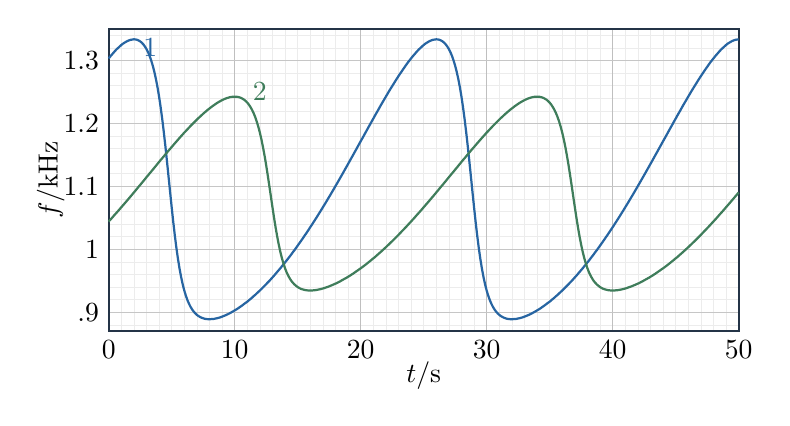
\begin{tikzpicture}[x=.16cm,y=8cm]
 \foreach\t in{0,1,...,50}{\draw[gray!15,very thin](\t,.87)--(\t,1.35);}
 \foreach\f in{.88,.90,...,1.34}{\draw[gray!15,very thin](0,\f)--(50,\f);}
 \foreach\t in{0,10,...,50}{\draw[gray!50](\t,.87)--(\t,1.35);\node[below]at(\t,.87){$\t$};}
 \foreach\f in{.9,1,1.1,1.2,1.3}{\draw[gray!45](0,\f)--(50,\f);\node[left]at(0,\f){$\f$};}
 \draw[body](0,.87)rectangle(50,1.35);
 \draw[blue,thick,domain=0:50,samples=401]plot(\x,{(16/15)/(1+.2*sqrt(2)*sin(15*\x-75)/sqrt(3-2*sqrt(2)*cos(15*\x-75)))});
 \draw[green,thick,domain=0:50,samples=401]plot(\x,{(16/15)/(1+.2/sqrt(2)*sin(15*\x-195)/sqrt(1.5-sqrt(2)*cos(15*\x-195)))});
 \node[blue,above]at(3.3,1.29){$1$};\node[green,above]at(12,1.22){$2$};
 \node[rotate=90]at(-4.6,1.11){$f/\mathrm{kHz}$};
 \node at(25,.80){$t/\mathrm s$};
\end{tikzpicture}
\begin{tikzpicture}
 \draw[vec](-.3,0)--(7,0)node[right]{传播方向};
 \fill[ink](0,0)circle(.05);\fill[red](1.2,0)circle(.05);
 \node[below]at(0,0){$S_0$};\node[below]at(1.2,0){$S_1$};
 \draw[vec](0,.6)--(1.2,.6)node[midway,above]{$u\,\Delta t_{\rm e}$};
 \draw[green,thick](5,-.5)--(5,.5);
 \draw[blue,thick](1.2,-.5)--(1.2,.5);
 \draw[dim](0,1.45)--(5,1.45)node[midway,above]{$c\,\Delta t_{\rm e}$};
 \draw[dim](1.2,-.95)--(5,-.95)node[midway,below]{$\lambda=(c-u)\Delta t_{\rm e}$};
 \node[green,right]at(5,.5){先发波前};
 \node[blue,below]at(1.2,-1.7){后一波前刚从 $S_1$ 发出};
 \draw[body](6,-.3)rectangle(6.45,.3);\node[above]at(6.2,.5){接收器};
\end{tikzpicture}
\begin{tikzpicture}
 \begin{scope}
 \coordinate(O)at(0,0);\coordinate(Q)at(2.2,0);\coordinate(P)at(-45:1.556);
 \draw[body](O)circle(1.556);
 \draw[body](O)--(Q)--(P)--cycle;
 \draw[vec](P)--({1.1+.6},{-1.1+.6})node[right]{$u=v$};
 \draw[body](1.1-.12,-1.1+.12)--(1.1,-1.1+.24)--(1.1+.12,-1.1+.12);
 \node[below left]at(O){$O$};\node[right]at(Q){$Q$外};\node[below]at(P){$P$};
 \node[below left]at(.55,-.55){$r$};\node[above]at(1.1,0){$b$};
 \end{scope}
 \begin{scope}[shift={(5.8,0)}]
 \coordinate(O)at(0,0);\coordinate(Q)at(1.1,0);\coordinate(P)at(-45:1.556);
 \draw[body](O)circle(1.556);
 \draw[body](O)--(Q)--(P)--cycle;
 \draw[vec](P)--({1.1+.7},{-1.1+.7})node[right]{$\boldsymbol v$};
 \draw[red,thick,-{Latex}](P)--(1.1,-.45)node[midway,left]{$u$};
 \draw[body](.9,0)--(.9,-.2)--(1.1,-.2);
 \node[below left]at(O){$O$};\node[above right]at(Q){$Q$内};\node[below]at(P){$P$};
 \node[below left]at(.55,-.55){$r$};\node[above]at(.55,0){$b$};
 \end{scope}
\end{tikzpicture}
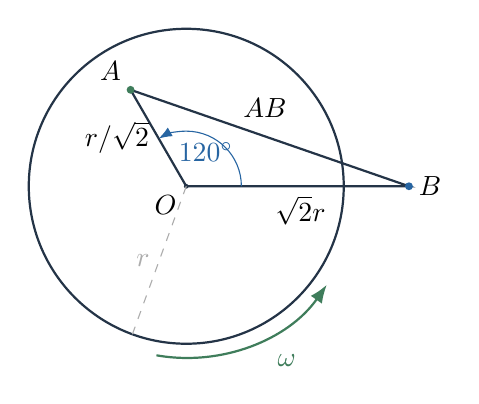
\begin{tikzpicture}
 \coordinate(O)at(0,0);\coordinate(A)at(120:{2/sqrt(2)});\coordinate(B)at({2*sqrt(2)},0);
 \draw[body](O)circle(2);
 \draw[body](O)--(A)--(B)--cycle;
 \fill[green](A)circle(.05);\fill[blue](B)circle(.05);
 \fill[ink](O)circle(.03);
 \node[below left]at(O){$O$};\node[above left]at(A){$A$};\node[right]at(B){$B$};
 \node[left]at(-.35,.62){$r/\sqrt2$};
 \node[below]at(1.45,0){$\sqrt2r$};
 \node[above]at(1,.75){$AB$};
 \draw[guide](O)--(250:2)node[midway,left]{$r$};
 \draw[blue,-{Latex}](.7,0)arc[start angle=0,end angle=120,radius=.7];
 \node[blue]at(60:.5){$120^\circ$};
 \draw[green,thick,-{Latex}](260:2.18)arc[start angle=260,end angle=325,radius=2.18];
 \node[green]at(300:2.55){$\omega$};
\end{tikzpicture}
\end{document}
